\documentclass[12pt,a4paper]{report}
\usepackage[utf8]{inputenc}
\usepackage[T1]{fontenc}
\usepackage[french]{babel}
\usepackage{graphicx}
\usepackage{geometry}
\usepackage{setspace}
\usepackage{hyperref}
\usepackage{titlesec}
\usepackage{xcolor}
\geometry{margin=2.5cm}
\usepackage{array}   % Pour personnaliser les colonnes
\usepackage[none]{hyphenat} % dans le préambule
\usepackage{float}

\onehalfspacing

\titleformat{\chapter}[display]
{\normalfont\bfseries\huge}{\chaptername\ \thechapter}{20pt}{\Huge}
\titleformat{\section}
{\normalfont\Large\bfseries}{\thesection}{1em}{}

\begin{document}
	
	\chapter*{Problématique}
	
	Dans le développement logiciel, la détection et la correction des erreurs représentent un défi majeur, notamment en raison de la diversité des sources d’anomalies (logs, stack traces, captures d’écran, retours utilisateurs, etc.) et de la complexité croissante des applications. Les méthodes traditionnelles de débogage reposent souvent sur une analyse manuelle, ce qui est chronophage et sujet à des erreurs humaines. De plus, les solutions existantes peinent à offrir une approche unifiée et intelligente pour interpréter ces anomalies et proposer des correctifs pertinents.
	
	L’absence d’un système capable de :
	
	\begin{itemize}
		\item Comprendre multimodalement les erreurs (texte, images, logs structurés).
		
		\item Proposer des corrections automatisées en s’appuyant sur des modèles de langage (LLMs) et des techniques de RAG (Retrieval-Augmented Generation).
		
		\item S’intégrer facilement dans des environnements DevOps existants.
	\end{itemize}
	
	rend ce projet particulièrement pertinent. Comment concevoir une application IA capable d’analyser efficacement ces différentes sources d’erreurs et de générer des solutions adaptées ?
	
	\chapter*{Objectifs}
	
	Ce projet vise à développer une application intelligente et modulaire permettant de détecter et corriger automatiquement les anomalies logicielles. Les objectifs spécifiques incluent :
	
	\begin{enumerate}
		\item Analyse Multimodale des Erreurs :
		\begin{itemize}
			\item Implémenter un système capable d’interpréter des données hétérogènes (stack traces, logs texte, captures d’écran, etc.).
			\item Utiliser des techniques de RAG pour enrichir les requêtes avec une base de connaissances (documentation technique, résolutions d’erreurs courantes).
		\end{itemize}
		
		\item Génération Automatique de Correctifs :
		\begin{itemize}
			\item Exploiter des LLMs (via Ollama) pour suggérer des corrections précises et contextualisées.
		\end{itemize}
		
		\item Intégration et Scalabilité :
		\begin{itemize}
			\item Développer un backend Spring Boot flexible, couplé à LangChain4J pour orchestrer les appels IA.
			
			\item Permettre une extension future via des connecteurs pour différents outils de monitoring.
		\end{itemize}
		
		\item Optimisation et Évaluation :
		\begin{itemize}
			\item Mesurer l’efficacité du système via des métriques de précision (taux de détection, pertinence des correctifs).
			
			\item Comparer avec des solutions existantes pour démontrer l’amélioration apportée.
		\end{itemize}
	\end{enumerate}
	
	\chapter{}

	\section{Langages, Frameworks et outils utilisés}
	
	\subsection{Java}
	
	\begin{figure}[H]
		\centering
		
\includegraphics[height=0.3\textwidth]{java-logo.png}
		\caption{Logo de Java}
		\label{fig:java-logo}
	\end{figure}
	
	Java est un langage de programmation orienté objet, robuste et multiplateforme, largement utilisé dans le développement d'applications d'entreprise. Sa forte typographie, sa gestion automatique de la mémoire (via le garbage collector) et son écosystème riche (bibliothèques, frameworks) en font un choix idéal pour les systèmes backend complexes.
	
	\subsection{Spring}
	
	\begin{figure}[H]
		\centering
		
\includegraphics[height=0.3\textwidth]{spring-logo.png}
		\caption{Logo de Spring}
		\label{fig:spring-logo}
	\end{figure}
	
	Spring est un framework modulaire pour Java, simplifiant le développement d'applications grâce à l’inversion de contrôle (IoC) et la programmation orientée aspect (AOP).
	
	\subsection{Spring Boot}
	
	\begin{figure}[H]
		\centering
		
\includegraphics[width=0.3\textwidth]{spring-boot-logo.png}
		\caption{Logo de Spring Boot}
		\label{fig:spring-boot-logo}
	\end{figure}
	
	Spring Boot étend Spring en fournissant des configurations automatiques, un serveur embarqué (Tomcat, Netty) et des outils clés en main (Spring Data, Spring Security), permettant de créer des applications standalone rapidement.
	
	\subsection{Maven}
	
	\begin{figure}[H]
		\centering
		
\includegraphics[width=0.3\textwidth]{maven-logo.png}
		\caption{Logo de Maven}
		\label{fig:maven-logo}
	\end{figure}
	
	Outil de build automatisé pour projets Java, qui gère Les dépendances (téléchargement auto), le packaging (JAR/WAR), et les cycles de compilation/test.
	
	\subsection{LangChain4j}
	
	\begin{figure}[H]
		\centering
		
\includegraphics[height=0.3\textwidth]{langchain4j-logo.png}
		\caption{Logo de LangChain4j}
		\label{fig:langchain4j-logo}
	\end{figure}
	
	LangChain4J est une bibliothèque Java inspirée de LangChain (Python), conçue pour intégrer facilement des LLMs (Modèles de Langage) dans des applications. Elle offre des abstractions pour la gestion des prompts, le RAG, les appels aux modèles (OpenAI, Ollama, etc.), et la connexion à des bases de données vectorielles.
	
	\subsection{Ollama}
	
	\begin{figure}[H]
		\centering
		
\includegraphics[height=0.3\textwidth]{ollama-logo.png}
		\caption{Logo de Ollama}
		\label{fig:ollama-logo}
	\end{figure}
	
	Ollama est un outil open-source permettant d’exécuter localement des LLMs (comme Llama 3, Mistral, Gemma) sans dépendre d’une API externe. Il est idéal pour prototyper des solutions IA offline, contrôler les coûts et la confidentialité des données, et personnaliser finement les modèles via des modelfiles.
	
	\subsection{IntelliJ IDEA}
	
	\begin{figure}[H]
		\centering
		
\includegraphics[height=0.3\textwidth]{intellij-logo.png}
		\caption{Logo de IntelliJ IDEA}
		\label{fig:intellij-logo}
	\end{figure}
	
	IntelliJ IDEA est un IDE puissant pour Java/Kotlin, développé par JetBrains. Ses avantages incluent une analyse intelligente du code (suggestions, détection d’erreurs), une intégration native avec Spring Boot et Maven/Gradle, des outils pour le débogage, le profiling et les tests, et des extensions pour l’IA (ex : GitHub Copilot).
	
	\section{Premier prototype}
	
	\subsection{Introduction}
	
	Pour atteindre cet objectif ambitieux, nous avons suivi une approche incrémentale. Dans un premier temps, un prototype fonctionnel a été réalisé afin de valider les fondements techniques du projet. Ce prototype est une application basée sur un agent intelligent exploitant une architecture RAG (Retrieval-Augmented Generation), capable de répondre aux questions de l’utilisateur à partir d’un document texte ou PDF fourni. Cette première version a permis de :
	\begin{itemize}
		\item comprendre le fonctionnement du framework LangChain4j ;
		\item tester l’intégration avec le LLM Ollama ;
		\item valider le concept de récupération de contexte à partir de documents externes.
	\end{itemize}
	
	\subsection{Fonctionnement d'un agent AI dans LangChain4j}
	
	Dans LangChain4j, un Agent AI orchestre les interactions entre un ChatLanguageModel (abstraction des LLMs comme OpenAI/Gemini/Ollama) et un ChatMemoryProvider (gestion de l'historique conversationnel). L'Agent formate les requêtes, intègre la mémoire contextuelle, et peut utiliser des outils externes, tandis que le LLM génère les réponses. Cette architecture modulaire permet une intégration flexible avec différents modèles et systèmes de stockage, tout en maintenant un état conversationnel cohérent.
	
	Le diagramme de séquences suivant décrit ce processus :
	
	\begin{figure}[H]
		\centering
		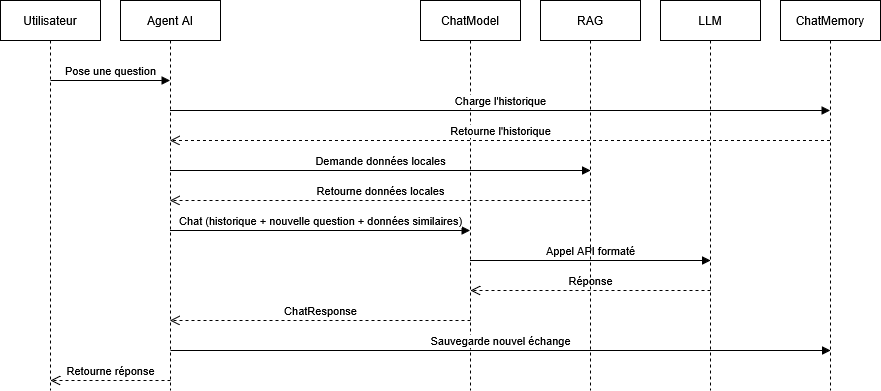
\includegraphics[width=\textwidth]{ds-ai-agent.drawio.png}
		\caption{Diagramme de séquences décrivant le fonctionnement d'un agent AI}
		\label{fig:ds-ai-agent.drawio}
	\end{figure}
	
	Le RAG combine deux phases clés pour améliorer la génération de réponses par un LLM : la rétroinformation (retrieval) et la génération contextuelle. Dans ce prototype, le système RAG :
	
	\begin{itemize}
		\item Charge d’abord un fichier source (texte, PDF, etc.).
		\item Utilise un DocumentPaser pour extraire les données brutes, et les découper en 'chunks'.
		\item Utilise un EmbeddingModel qui convertit ces chunks en vecteurs d’embedding (représentations numériques sémantiques).
		\item Utilise un EmbeddingStoreIngestor pour stocker ces vecteurs dans un EmbeddingStore.
		\item Utilise un Retriever qui interroge l’EmbeddingStore pour trouver les documents les plus pertinents par rapport à la question de l'utilisateur.
	\end{itemize}
	
	Le diagramme de séquences suivant détaille ces étapes :
	
	\begin{figure}[H]
		\centering
		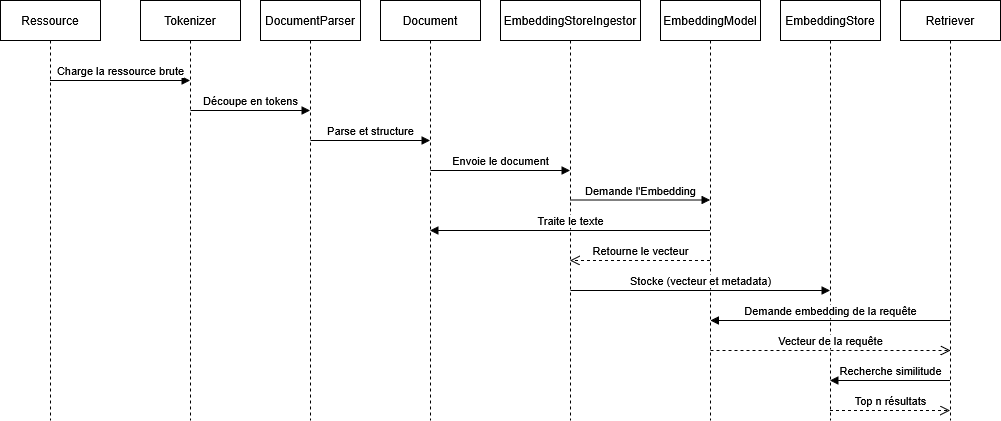
\includegraphics[width=\textwidth]{ds-rag.drawio.png}
		\caption{Diagramme de séquences décrivant le fonctionnement du RAG}
		\label{fig:ds-rag.drawio}
	\end{figure}
	
	Pour tester ce prototype, nous avons fourni un fichier PDF, son contenu est une lettre de recommandation pour une étudiante appelée Nour, on a ensuite envoyé une question à propos de cette étudiante à l'agent AI, en utilisant un contrôleur web :
	
	\begin{figure}[H]
		\centering
		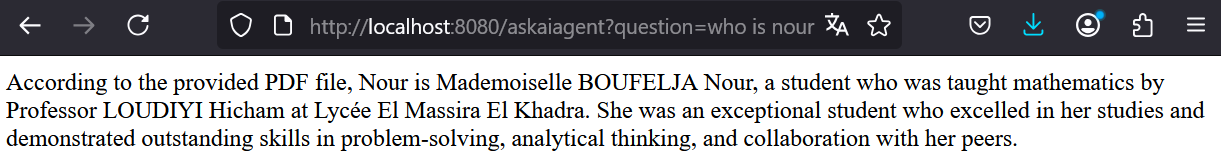
\includegraphics[width=\textwidth]{test-rag.png}
		\caption{Test du RAG}
		\label{fig:test-rag}
	\end{figure}
	
	
	
\end{document}}